% ========================================
%	Header einbinden
% ========================================

\documentclass[bibtotoc,titlepage]{scrartcl}

% Deutsche Spracheinstellungen
\usepackage[ngerman,german]{babel, varioref}
\usepackage[T1]{fontenc}
\usepackage[utf8]{inputenc}

%\usepackage{marvosym}

\usepackage{amsfonts}
\usepackage{amssymb}
\usepackage{amsmath}
\usepackage{amscd}
\usepackage{amstext}
\usepackage{float}
\usepackage{caption}
\usepackage{wrapfig}
\usepackage{setspace}
\usepackage{threeparttable}
\usepackage{footnote}

\usepackage{caption}
\usepackage{subcaption}

\newfloat{formel}{htbp}{for}
\floatname{formel}{Formel}


\usepackage{longtable}

%\usepackage{bibgerm}

\usepackage{footnpag}

\usepackage{ifthen}                 %%% package for conditionals in TeX
\usepackage{siunitx}
%Fr textumflossene Bilder und Tablellen
%\usepackage{floatflt} - veraltet

%Fr Testzwecke aktivieren, zeigt labels und refs im Text an.
%\usepackage{showkeys}

% Abstand zwischen zwei Abs�zen nach DIN (1,5 Zeilen)
% \setlength{\parskip}{1.5ex plus0.5ex minus0.5ex}

% Einrckung am Anfang eines neuen Absatzes nach DIN (keine)
%\setlength{\parindent}{0pt}

% R�der definieren
% \setlength{\oddsidemargin}{0.3cm}
% \setlength{\textwidth}{15.6cm}

% bessere Bildunterschriften
%\usepackage[center]{caption2}


% Probleml�ungen beim Umgang mit Gleitumgebungen
\usepackage{float}

% Nummeriert bis zur Strukturstufe 3 (also <section>, <subsection> und <subsubsection>)
%\setcounter{secnumdepth}{3}

% Fhrt das Inhaltsverzeichnis bis zur Strukturstufe 3
%\setcounter{tocdepth}{3}

\usepackage{exscale}

\newenvironment{dsm} {\begin{displaymath}} {\end{displaymath}}
\newenvironment{vars} {\begin{center}\scriptsize} {\normalsize \end{center}}


\newcommand {\en} {\varepsilon_0}               % Epsilon-Null aus der Elektrodynamik
\newcommand {\lap} {\; \mathbf{\Delta}}         % Laplace-Operator
\newcommand {\R} { \mathbb{R} }                 % Menge der reellen Zahlen
\newcommand {\e} { \ \mathbf{e} }               % Eulersche Zahl
\renewcommand {\i} { \mathbf{i} }               % komplexe Zahl i
\newcommand {\N} { \mathbb{N} }                 % Menge der nat. Zahlen
\newcommand {\C} { \mathbb{C} }                 % Menge der kompl. Zahlen
\newcommand {\Z} { \mathbb{Z} }                 % Menge der kompl. Zahlen
\newcommand {\limi}[1]{\lim_{#1 \rightarrow \infty}} % Limes unendlich
\newcommand {\sumi}[1]{\sum_{#1=0}^\infty}
\newcommand {\rot} {\; \mathrm{rot} \,}         % Rotation
\newcommand {\grad} {\; \mathrm{grad} \,}       % Gradient
\newcommand {\dive} {\; \mathrm{div} \,}        % Divergenz
\newcommand {\dx} {\; \mathrm{d} }              % Differential d
\newcommand {\cotanh} {\; \mathrm{cotanh} \,}   %Cotangenshyperbolicus
\newcommand {\asinh} {\; \mathrm{areasinh} \,}  %Area-Sinus-Hyp.
\newcommand {\acosh} {\; \mathrm{areacosh} \,}  %Area-Cosinus-H.
\newcommand {\atanh} {\; \mathrm{areatanh} \,}  %Area Tangens-H.
\newcommand {\acoth} {\; \mathrm{areacoth} \,}  % Area-cotangens
\newcommand {\Sp} {\; \mathrm{Sp} \,}
\newcommand {\mbe} {\stackrel{\text{!}}{=}}     %Must Be Equal
\newcommand{\qed} { \hfill $\square$\\}
\renewcommand{\i} {\imath}
\def\captionsngerman{\def\figurename{\textbf{Abb.}}}

%%%%%%%%%%%%%%%%%%%%%%%%%%%%%%%%%%%%%%%%%%%%%%%%%%%%%%%%%%%%%%%%%%%%%%%%%%%%
% SWITCH FOR PDFLATEX or LATEX
%%%%%%%%%%%%%%%%%%%%%%%%%%%%%%%%%%%%%%%%%%%%%%%%%%%%%%%%%%%%%%%%%%%%%%%%%%%%
%%%
\ifx\pdfoutput\undefined %%%%%%%%%%%%%%%%%%%%%%%%%%%%%%%%%%%%%%%%% LATEX %%%
%%%
\usepackage[dvips]{graphicx}       %%% graphics for dvips
\DeclareGraphicsExtensions{.eps,.ps}   %%% standard extension for included graphics
\usepackage[ps2pdf]{thumbpdf}      %%% thumbnails for ps2pdf
\usepackage[ps2pdf,                %%% hyper-references for ps2pdf
bookmarks=true,%                   %%% generate bookmarks ...
bookmarksnumbered=true,%           %%% ... with numbers
hypertexnames=false,%              %%% needed for correct links to figures !!!
breaklinks=true,%                  %%% breaks lines, but links are very small
linkbordercolor={0 0 1},%          %%% blue frames around links
pdfborder={0 0 112.0}]{hyperref}%  %%% border-width of frames
%                                      will be multiplied with 0.009 by ps2pdf
%
%\hypersetup{ pdfauthor   = {Hannes Franke; Julius Tilly},
%pdftitle    = {x}, pdfsubject  = {Protokoll FP}, pdfkeywords = {V301, Innenwiderstand, Leistungsanpassung},
%pdfcreator  = {LaTeX with hyperref package}, pdfproducer = {dvips
%+ ps2pdf} }
%%%
\else %%%%%%%%%%%%%%%%%%%%%%%%%%%%%%%%%%%%%%%%%%%%%%%%%%%%%%%%%% PDFLATEX %%%
%%%
\usepackage[pdftex]{graphicx}      %%% graphics for pdfLaTeX
\DeclareGraphicsExtensions{.pdf}   %%% standard extension for included graphics
\usepackage[pdftex]{thumbpdf}      %%% thumbnails for pdflatex
\usepackage[pdftex,                %%% hyper-references for pdflatex
bookmarks=true,%                   %%% generate bookmarks ...
bookmarksnumbered=true,%           %%% ... with numbers
hypertexnames=false,%              %%% needed for correct links to figures !!!
breaklinks=true,%                  %%% break links if exceeding a single line
linkbordercolor={0 0 1},
linktocpage]{hyperref} %%% blue frames around links
%                                  %%% pdfborder={0 0 1} is the default
% \hypersetup{
% pdftitle    = {V301 Innenwiderstand und Leistungsanpassung}, 
% pdfsubject  = {Protokoll AP}, 
% pdfkeywords = {V301, Innenwiderstand, Leistungsanpassung},
% pdfsubject  = {Protokoll AP},
% pdfkeywords = {V301, Innenwiderstand, Leistungsanpassung}}
%                                  %%% pdfcreator, pdfproducer,
%                                      and CreationDate are automatically set
%                                      by pdflatex !!!
\pdfadjustspacing=1                %%% force LaTeX-like character spacing
\usepackage{epstopdf}
%
\fi %%%%%%%%%%%%%%%%%%%%%%%%%%%%%%%%%%%%%%%%%%%%%%%%%%% END OF CONDITION %%%
%%%%%%%%%%%%%%%%%%%%%%%%%%%%%%%%%%%%%%%%%%%%%%%%%%%%%%%%%%%%%%%%%%%%%%%%%%%%
% seitliche Tabellen und Abbildungen
%\usepackage{rotating}
\usepackage{ae}
\usepackage{
  array,
  booktabs,
  dcolumn
}
\makeatletter 
  \renewenvironment{figure}[1][] {% 
    \ifthenelse{\equal{#1}{}}{% 
      \@float{figure} 
    }{% 
      \@float{figure}[#1]% 
    }% 
    \centering 
  }{% 
    \end@float 
  } 
  \makeatother 


  \makeatletter 
  \renewenvironment{table}[1][] {% 
    \ifthenelse{\equal{#1}{}}{% 
      \@float{table} 
    }{% 
      \@float{table}[#1]% 
    }% 
    \centering 
  }{% 
    \end@float 
  } 
  \makeatother 
%\usepackage{listings}
%\lstloadlanguages{[Visual]Basic}
%\allowdisplaybreaks[1]
%\usepackage{hycap}
%\usepackage{fancyunits}
\sisetup{output-decimal-marker = {,}}

% ========================================
%	Angaben für das Titelblatt
% ========================================

\title{V01 - Lebensdauer der Myonen\\				% Titel des Versuchs 
\large TU Dortmund, Fakultät Physik\\ 
\normalsize Fortgeschrittenen-Praktikum}

\author{Jan Latarius\\			% Name Praktikumspartner A
{\small \href{jan.latarius@tu-dortmund.de}{jan.latarius@tu-dortmund.de}}	% Erzeugt interaktiven einen Link
\and						% um einen weiteren Author hinzuzfügen
Dimitrios Skodras\\					% Name Praktikumspartner B
{\small \href{dimitrios.skodras@tu-dortmund.de}{dimitrios.skodras@tu-dortmund.de}}		% Erzeugt interaktiven einen Link
}
\date{19.12.2016}				% Das Datum der Versuchsdurchführung

% ========================================
%	Das Dokument beginnt
% ========================================

\begin{document}

% ========================================
%	Titelblatt erzeugen
% ========================================

\maketitle					% Jetzt wird die Titelseite erzeugt
\thispagestyle{empty} 				% Weder Kopfzeile noch Fußzeile

% ========================================
%	Der Vorspann
% ========================================

%\newpage					% Wenn Verzeichnisse auf einer neuen Seite beginnen sollen
%\pagestyle{empty}				% Weder Kopf- noch Fußzeile für Verzeichnisse

\tableofcontents

%\newpage					% eine neue Seite
%\thispagestyle{empty}				% Weder Kopf- noch Fußzeile für Verzeichnisse
%\listoffigures					% Abbildungsverzeichnis

%\newpage					% eine neue Seite
%\thispagestyle{empty}				% Weder Kopf- noch Fußzeile für Verzeichnisse
%\listoftables					% Tabellenverzeichnis
\newpage					% eine neue Seite


% ========================================
%	Kapitel
% ========================================

%\section{Einleitung}				% Bei Bedarf

\section{Theorie}

\section{Durchführung}
\label{sec:exec}

\section{Auswertung}
\subsection{Verzögerungsleitung}
Wie in Abbildung \ref{pic:setup} dargestellt und in Abschnitt \ref{sec:exec} beschrieben, soll gewährleistet werden, dass die Signale der SEVs 
gleichzeitig zur Koinzidenzapparatur gelangen. Die Verzögerung erreicht mit hinzukommender Kabellänge sowie ihr Einfluss auf die Signalrate
sind in Tabelle \ref{tab:koinz} aufgeführt. Man erkennt eine relativ geringe Einflussnahme der Verzögerung entsprechend des breiten Plateaus,
weshalb angenommen wird, dass der tatsächlichen Wahl eine gewisse Freiheit beiwohnt. 
Während der Versuchsdurchführung ist die Verzögungsleitung auf \SI{-3}{\nano\second} angestellt worden, da die abfallenden Flanken an den 
Rändern der Messreihe darum zentriert sind. 
\begin{table}[b]
\input{../auswertung/koinzidenz.dat}
\caption{Verzögerungsleitung zur Synchronisierung der SEVs. Negative $t$ entsprechen einer Verzögerung des linken SEVs. In der dritten Spalte 
sind die Zählraten auf 10\,s Messzeit aufgeführt.}
\label{tab:koinz}
\end{table}
Entsprechend des Myonenstroms \cite{pdg} werden die Diskriminatoren einer Rate von 20-30\,\si{\per\second} entsprechend eingestellt. Die 
Pulsbreite wird am Oszillator zu \SI{11,5}{\s} abgelesen.
\subsection{Kalibrierung der Zeitachse}
Die Zeitdifferenz $\Delta t$ zwischen zwei vom Doppelimpulsgenerator Signalen wird vom TAC in eine Spannung umgewandelt, die vom Vielkanalanalysator 
ausgelesen wird. Diese Differenz wird in \SI{1}{\nano\second}-Schritten von \SI{1}{\nano\second} bis \SI{9}{\nano\second} variiert und geprüft,
welchem Kanal sie zugeordnet wird \footnote{Aufgrund eines mutmaßlichen, technischen Fehlers des TACs sind die zur weiteren Auswertung benötigten
Daten vom Versuchsbetreuer \href{robert.theinert@tu-dortmund.de}{Robert Theinert} gestellt worden.}. Der sich abzeichnende lineare Zusammenhang
\begin{align}
 f(x) = ax + b
\end{align}
ist in Abbildung \ref{pic:linfit} 
\begin{figure}[t]
 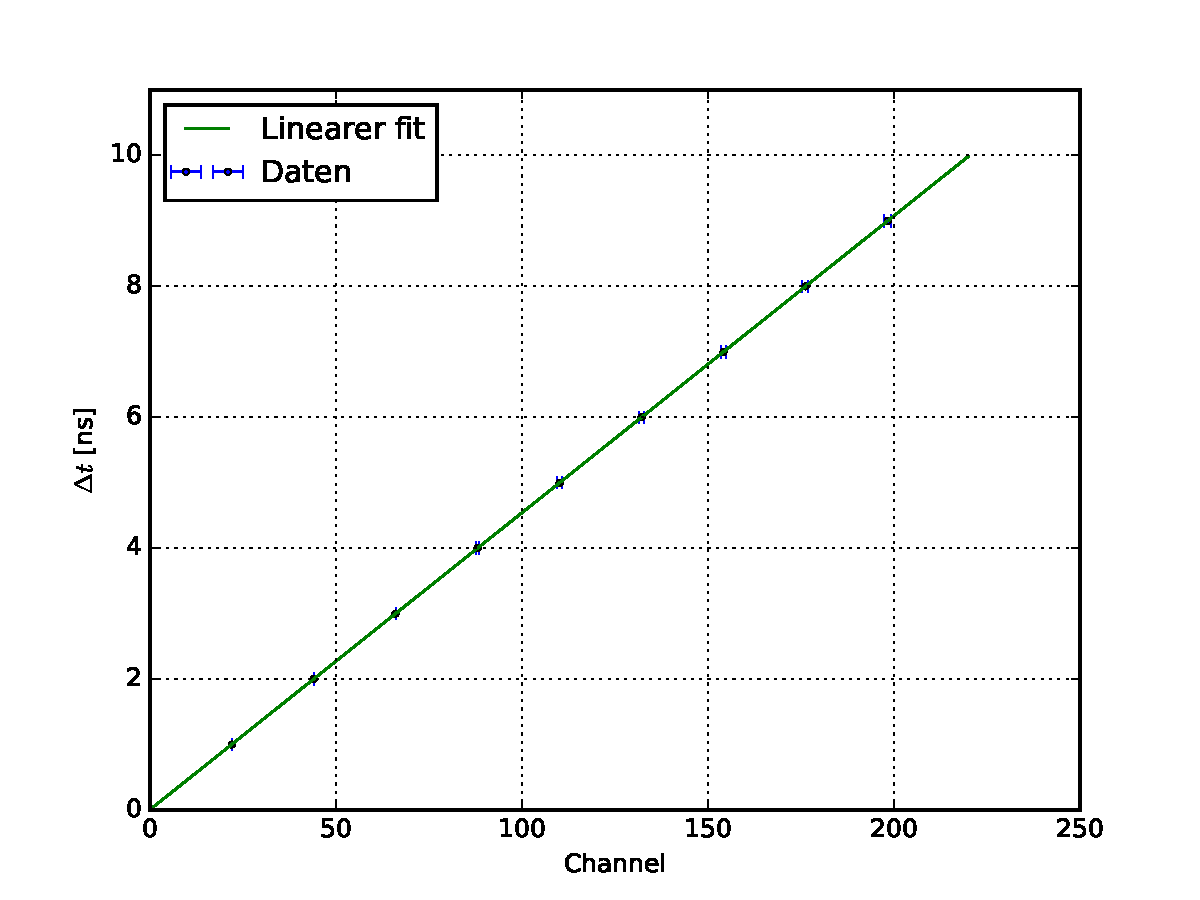
\includegraphics[width=0.7\textwidth]{../pics/linFit}
 \caption{}
 \label{pic:linfit}
\end{figure}
dargestellt und seine Fitparameter, bestimmt durch \texttt{Python3.6}, ergeben sich zu
\begin{align}
 a&= \SI{4,54(1)e-2}{\nano\second\per Kanal}\\
 b&= \SI{5,50(1)e-3}{\nano\second}.
 \label{eq:kalibparams}
\end{align}
Die Berechnung bezieht nur die ersten 200 Kanäle mit ein, jedoch sind 512 vorhanden, weshalb der lineare Zusammenhang aufgrund des kleinen Fehlers
fortgeführt wird.
Es kommt beim Auslesen teilweise zu einer Zuordnung auf mehrere, direkt nebeneinanderliegende Kanäle sodass ein gewichtetes Mittel verwandt wird.
Der dadurch entstehende Fehler hat einen verschwindenden Einfluss auf die Fitparameter. Weiterhin gibt es Fälle, in denen kleine Fluktuationen
von einem Count in einem beliebigen Kanal auftauchen. Diese werden nicht berücksichtigt.
\subsection{Bestimmung der Untergrundrate}
Während einer Messzeit von $t_\text{mess}=\SI{1449146}{\second}$ werden $N_\text{start}=\SI{32201706}{}$ Anfangsimpulse gezählt, was einer Rate von 
\begin{align}
 \bar N = \frac{N_\text{start}}{t_\text{mess}} = \SI{22,22(1)}{\per\second}
\end{align}
entspricht. Dies liegt im erwarteten Bereich, was darauf schließen lässt, dass die meisten Untergrundsignale von den Diskriminatoren herausgefiltert
worden sind. Während der Suchzeit $t_S=\SI{22}{\mu\second}$ kann ein zweites Myon in den Tank eintreten. Das daherrührende Untergrundsignal kann
mit der Poisson-Verteilung abgeschätzt werden. Dass genau ein weiteres Myon eintritt, entspricht einer Wahrscheinlichkeit von
\begin{align}
 P(n=1) = \bar N t_S \e^{-\bar N t_S} = \SI{4,886(1)e-4}{},
\end{align}
sodass also 
\begin{align}
 N_b = P(n=1)N_\text{start} = \SI{15735(6)}{}.
\end{align}
Hintergrundsignale sich gleichmäßig auf die Kanal mit $\Delta t < t_S$ verteilen. Aus \eqref{eq:kalibparams} ergibt sich die Anzahl beteiligter 
Kanäle zu
\begin{align}
 \text{Kanal}_\text{max} = t_S\frac{1}{a} - \frac{b}{a}  = 484,84(1),
\end{align}
womit die Untergrundsignale
\begin{align}
 U_\text{erw} = \frac{N_b}{\text{Kanal}_\text{max}} = \SI{32,45(1)}{1\per Kanal}
\end{align}
zu erwarten sind.
\subsection{Bestimmung der Lebensdauer von Myonen}


\begin{figure}[t]
 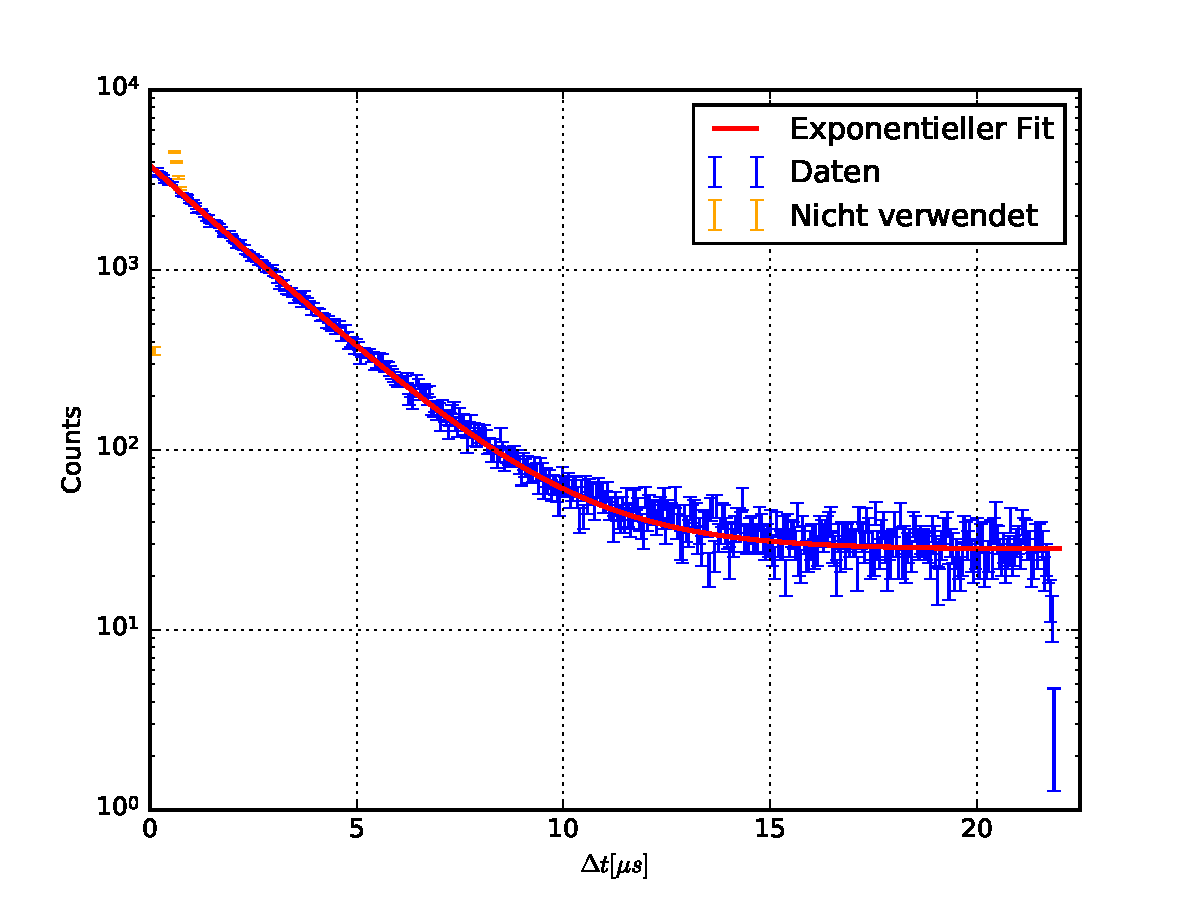
\includegraphics[width=0.8\textwidth]{../pics/lebensdauer_fit}
 \caption{}
 \label{pic:lebensdauer}
\end{figure}



%\parskip 340pt
%\Large{Literatur}\\\\
\newpage
 \begin{thebibliography}{WissOnl}
 	\bibitem{Anl} TU Dortmund Anleitung für Versuch Nr.01 \url{http://129.217.224.2/HOMEPAGE/Anleitung_FPBSc.html}
 	\bibitem{pdg} C. Patrignani et al. (Particle Data Group), Chin. Phys. C, 40, 100001 (2016).
	\end{thebibliography}

% ========================================
%	Literaturverzeichnis
% ========================================

%\bibliographystyle{plainnat}			% Bibliographie-Style auswählen
%\bibliography{BIBDATEI}			% Literaturverzeichnis

% ========================================
%	Das Dokument endent
% ========================================

\end{document}
